% Commands for Plots
% outdated (from TACAS)
\newcommand{\numqvbsfull}{366}
\newcommand{\numqvbshard}{18}


\newcommand{\numcommunity}{80}
\newcommand{\numpremise}{200}
\newcommand{\numalljani}{449}
\newcommand{\numhard}{117}
\newtoggle{showplots}
 \toggletrue{showplots}
% \togglefalse{showplots}
 % \usepackage{showframe}

%% Colours
\definecolor{plotred}{RGB}{255,0,0}
\definecolor{plotgreen}{RGB}{0,255,0}
\definecolor{plotblue}{RGB}{0,0,255}
\definecolor{plotyellow}{RGB}{230,230,0}
\definecolor{plotcyan}{RGB}{0,255,255}
\definecolor{plotorange}{RGB}{255,127,0}
\definecolor{plotpink}{RGB}{255,0,255}
\definecolor{plotlightgray}{RGB}{192,192,192}
\definecolor{plotdarkgray}{RGB}{128,128,128}
\definecolor{plotdarkred}{RGB}{128,0,0}
\definecolor{plotgreenyellow}{RGB}{128,128,0}
\definecolor{plotdarkgreen}{RGB}{0,128,0}
\definecolor{plotpurple}{RGB}{128,0,128}
\definecolor{plotteal}{RGB}{0,128,128}
\definecolor{plotdarkblue}{RGB}{0,0,128}
\definecolor{plotlightred}{RGB}{205,92,92}
\definecolor{plotlightblue}{RGB}{176,196,222}
\colorlet{color1}{plotred}
\colorlet{color2}{plotgreen}
\colorlet{color3}{plotblue}
\colorlet{color4}{plotyellow}
\colorlet{color5}{plotcyan}
\colorlet{color6}{plotorange}
\colorlet{color7}{plotpink}
\colorlet{color8}{plotlightgray}
\colorlet{color9}{plotdarkgray}
\colorlet{color10}{plotdarkred}
\colorlet{color11}{plotgreenyellow}
\colorlet{color12}{plotdarkgreen}
\colorlet{color13}{plotpurple}
\colorlet{color14}{plotteal}
\colorlet{color15}{plotdarkblue}
\colorlet{color16}{plotlightred}
\colorlet{color17}{plotlightblue}

\colorlet{colmcstavi}{color1}
\colorlet{colmcstaovi}{color11}
\colorlet{colstormvi}{color3}
\colorlet{colstormovi}{color7}
\colorlet{colstormpi}{color14}
\colorlet{colstormlp}{color6}



%% Quantileplots
\newcommand{\quantileplotxlabel}{solved benchmarks}
\newcommand{\quantileplotylabel}{runtime}
\newlength{\quantileplotwidth}
\newlength{\quantileplotheight}
\setlength{\quantileplotwidth}{0.5\linewidth}
\setlength{\quantileplotheight}{0.5\linewidth}
\newcommand{\quantileplotlegendcols}{1}

\newcommand{\standardquantileplotlinestyle}{ultra thick}
\newcommand{\quantileplotlinestyle}{\standardquantileplotlinestyle}

\newcommand{\quantileplot}[8]{%
% Arguments:
% #1: csv filename
% #2: comma separated list of tool.config/color items}
% #3: comma separated list of readable config names 
% #4: xmin
% #5: xmax
% #6: ymin
% #7: ymax
% #8: legend pos (e.g. "north west")
	\begin{tikzpicture}
	\begin{axis}[
	width=\quantileplotwidth,
	height=\quantileplotheight,
	xmin=#4,
	xmax=#5,
	ymin=#6,
	ymax=#7,
	ymajorgrids,
	ymode=log,
	axis x line=bottom,
	axis y line=left,
	unbounded coords=discard,filter discard warning=false, % properly deal with missing data points
	% ytick= {1, 6, 60, 600, 1200, 1800 },
	% yticklabels={$\le$1, 6, 60, 600, 1200, 1800},
	xlabel=\quantileplotxlabel,
	xlabel style={font=\scriptsize,yshift=4pt},%{yshift=16pt},
	ylabel=\quantileplotylabel,
	ylabel style={font=\scriptsize,yshift=-7pt},%{yshift=-0.4cm},
	log ticks with fixed point, % enable to avoid 10^-x notation
	yticklabel style={font=\scriptsize},
	scaled y ticks=false,
	xticklabel style={font=\scriptsize},
	legend columns=\quantileplotlegendcols,
	legend pos={#8},
	legend style={nodes={scale=0.75, transform shape},inner sep=1pt},
/pgfplots/legend image code/.code={\draw[mark repeat=2,mark phase=2,##1] plot coordinates {(0cm,0cm) (0.3cm,0cm)};}, % make the legend lines a bit smaller
	every axis plot/.append style={\quantileplotlinestyle},
	legend cell align={left}
	]
	\iftoggle{showplots}{
	\foreach \tool\color in {#2}{%
		\edef\loopbody{
			\noexpand\addplot[\color] table [x=n,y=\tool shifted, col sep=tab] {#1};
		}
		\loopbody
	}
	\legend{#3}}{\node[anchor=south west, align=center, red] {\huge NOT\\ COMPILED};}
	\end{axis}
	\end{tikzpicture}%
}


%% Scatter plots
\newlength\scatterplotsize
\setlength{\scatterplotsize}{0.365\linewidth}
\newcommand{\scatterplot}[6]{%
% Arguments:
% #1: csv filename
% #2: tool.config identifier for x-axis
% #3: label for x-axis
% #4: tool.config identifier for y-axis
% #5: label for y-axis
% #6: trigger showing the legend (true/false)
	\begin{tikzpicture}
	\begin{axis}[
	width=\scatterplotsize,
	height=\scatterplotsize,
	axis equal image,
	xmin=1,
	ymin=1,
	ymax=1280,
	xmax=1280,
	xmode=log,
	ymode=log,
	axis x line=bottom,
	axis y line=left,
	xtick={2,4,8,16,32,64,128,256},
	xticklabels={2,4,8,16,,64,,\!\!256},
	extra x ticks = {1,512,724},
	extra x tick labels = {${\le}1$,,\,\,n/a},
	extra x tick style = {grid = major},
	ytick={2,4,8,16,32,64,128,256},
	yticklabels={2,4,8,16,32,64,,},
	extra y ticks = {1,512,724},
	extra y tick labels = {${\le}1$,$\ge$512},
	extra y tick style = {grid = major},
	xlabel={#3},
	xlabel style={font=\scriptsize,yshift=5pt},%{yshift=16pt},
	ylabel={#5},
	ylabel style={font=\scriptsize,yshift=-9pt},%{yshift=-0.4cm},
	yticklabel style={font=\scriptsize},
	xticklabel style={font=\scriptsize},%rotate=290,anchor=west,
	legend pos=north east,
	legend columns=3,
	legend style={nodes={scale=0.75, transform shape},inner sep=1.5pt, xshift=1mm, yshift=7mm},
	set layers,
	mark layer=axis background
	%legend cell align={left}
	]
	
	\iftoggle{showplots}{\addplot[
	scatter,
	only marks,
	scatter/classes={
		maqvbs={mark=diamond*,color1,mark size=1.75},
		ptaqvbs={mark=pentagon*,color3,mark size=1.75},
		mdpqvbs={mark=triangle*,color2,mark size=1.75},
		mdpmec={mark=asterisk,color7,mark size=1.75},
		mdpgrid={mark=*,color5,mark size=1.75},
		mdpgridmec={mark=otimes,color6,mark size=1.75}
	},
	scatter src=explicit symbolic
	]%
	table [col sep=tab,x=#2,y=#4,meta=Class] {#1};
	}{\node[anchor=south west, align=center, red] {\huge NOT\\ COMPILED};}
	\ifthenelse{\NOT\equal{#6}{false}}{\legend{MA,PTA,MDP$_\mathit{qvbs}$,MDP$^\mathit{mec}$,MDP$_\mathit{grid}$,MDP$_\mathit{grid}^\mathit{mec}$}}{}
	\addplot[no marks] coordinates {(0.01,0.01) (512,512) };
	\addplot[no marks, densely dotted] coordinates {(0.01,0.02) (256,512)};
	\addplot[no marks, densely dotted] coordinates {(0.02,0.01) (512,256)};
	\end{axis}
	\end{tikzpicture}
}


\newcommand{\hardwarquantileplot}[7]{
% Arguments:
% #1: csv filename
% #2: hardware-config-name
% #4: xmin
% #5: xmax
% #6: ymin
% #7: ymax
% #8: legend pos (e.g. "north west")
\renewcommand{\quantileplotlinestyle}{thick}%
\quantileplot{#1}{#2.Storm.ovi-topo/colstormovi,#2.Storm.vi-topo/colstormvi,#2.mcsta.ovi/colmcstaovi,#2.mcsta.vi/colmcstavi,#2.Storm.vi2pi-topo-gmres/colstormpi,#2.Storm.vi2lp-topo-gurobi/colstormlp}{
%$\text{OVI}_\tool{s}$, $\text{VI}_\tool{s}$, $\text{OVI}_\tool{m}$, $\text{VI}_\tool{m}$,$\text{VI2PI}_\tool{s}$,  $\text{VI2LP}_\tool{s}$
}{#3}{#4}{#5}{#6}{#7}
% Arguments:
% #1: csv filename
% #2: comma separated list of tool.config/color items}
% #3: comma separated list of readable config names 
% #4: xmin
% #5: xmax
% #6: ymin
% #7: ymax
% #8: legend pos (e.g. "north west")
\renewcommand{\quantileplotlinestyle}{\standardquantileplotlinestyle} %
}

\colorlet{colclaix23}{red}
\colorlet{cole1620}{blue!50!white}
\colorlet{colR32200}{green!80!white}
\colorlet{colR54650U}{green!60!black}
\colorlet{colR97950}{green!80!black}
\colorlet{colTRP5965}{green!60!yellow!30!black}
\colorlet{coli910980}{blue!80!white}
\colorlet{coli911900}{blue!90!black}

\colorlet{colM2Pro}{brown}

\newcommand{\hardwarmethodsquantileplot}[7]{
% Arguments:
% #1: csv filename
% #2: method-name
% #4: xmin
% #5: xmax
% #6: ymin
% #7: ymax
% #8: legend pos (e.g. "north west")
\renewcommand{\quantileplotlinestyle}{thick}%
\quantileplot{#1}{logs-E1620-dockerized.#2/cole1620,logs-R32200-dockerized.#2/colR32200,logs-R54650U-dockerized.#2/colR54650U,logs-R97950X-dockerized.#2/colR97950,logs-i910980xe-dockerized.#2/coli910980,logs-M2Pro.#2/colM2Pro,logs-TRP5965-dockerized.#2/colTRP5965,logs-i911900K-dockerized.#2/coli911900,logs-claix23.#2/colclaix23
}{%claix23,E1620,R32200,R54650U,R97950X,TRP5965,i910980,i911900
}{#3}{#4}{#5}{#6}{#7}%
% Arguments:
% #1: csv filename
% #2: comma separated list of tool.config/color items}
% #3: comma separated list of readable config names 
% #4: xmin
% #5: xmax
% #6: ymin
% #7: ymax
% #8: legend pos (e.g. "north west")
\renewcommand{\quantileplotlinestyle}{\standardquantileplotlinestyle} %
}
\newcommand{\hardwaremethodslegend}{
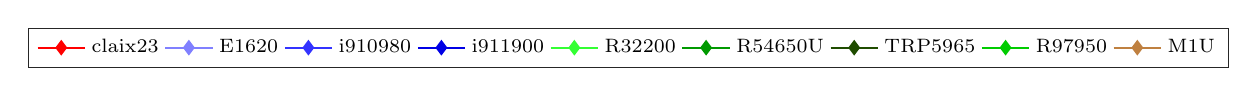
\begin{tikzpicture}
\begin{axis}[width=0.8\textwidth, height=0.2\textwidth, hide axis, xmin=0, xmax=10, ymin=0, ymax=0.2,legend columns=9, 
            legend style={draw=white!15!black,legend cell align=left, at={(0.5,0.5), font=\scriptsize}},]
%    \foreach \toolname/\tcolor in {claix23/colclaix23,E1620/cole1620,i910980xe/coli910980,i911900K/coli911900,R32200/colR32200,R54650U/colR54650U,TRP5965/colTRP5965,R97950X/colR97950}{
%		\edef\loopbody{
%			\noexpand\addlegendimage{\tcolor, mark=diamond*, thick, mark options={solid,scale=1.1}}\noexpand\addlegendentry{\toolname}
%   % what
%		}
%		\show\loopbody
%		\loopbody
%	}
	% claix23/colclaix23,E1620/cole1620,i910980xe/coli910980,i911900K/coli911900,R32200/colR32200,R54650U/colR54650U,TRP5965/colTRP5965,R97950X/colR97950
	\addlegendimage{colclaix23, mark=diamond*, thick, mark options={solid,scale=1.1}}
	\addlegendentry{claix23}
	
	\addlegendimage{cole1620, mark=diamond*, thick, mark options={solid,scale=1.1}}
	\addlegendentry{E1620}
	
	\addlegendimage{coli910980, mark=diamond*, thick, mark options={solid,scale=1.1}}
	\addlegendentry{i910980}
	
	\addlegendimage{coli911900, mark=diamond*, thick, mark options={solid,scale=1.1}}
	\addlegendentry{i911900}
	
	\addlegendimage{colR32200, mark=diamond*, thick, mark options={solid,scale=1.1}}
	\addlegendentry{R32200}
	
	\addlegendimage{colR54650U, mark=diamond*, thick, mark options={solid,scale=1.1}}
	\addlegendentry{R54650U}
	
	\addlegendimage{colTRP5965, mark=diamond*, thick, mark options={solid,scale=1.1}}
	\addlegendentry{TRP5965}
	
	\addlegendimage{colR97950, mark=diamond*, thick, mark options={solid,scale=1.1}}
	\addlegendentry{R97950}
	
	\addlegendimage{colM2Pro, mark=diamond*, thick, mark options={solid,scale=1.1}}
	\addlegendentry{M1U}
	
    \end{axis}
\end{tikzpicture}
}

\newcommand{\hardwarescatterplot}[6]{%
% Arguments:
% #1: csv filename
% #2: tool.config identifier for x-axis
% #3: label for x-axis
% #4: tool.config identifier for y-axis
% #5: label for y-axis
% #6: trigger showing the legend (true/false)
	\begin{tikzpicture}
	\begin{axis}[
	width=\scatterplotsize,
	height=\scatterplotsize,
	axis equal image,
	xmin=1,
	ymin=1,
	ymax=1280,
	xmax=1280,
	xmode=log,
	ymode=log,
	axis x line=bottom,
	axis y line=left,
	xtick={2,4,8,16,32,64,128,256},
	xticklabels={2,4,8,16,,64,,\!\!256},
	extra x ticks = {1,512,724},
	extra x tick labels = {${\le}1$,,\,\,n/a},
	extra x tick style = {grid = major},
	ytick={2,4,8,16,32,64,128,256},
	yticklabels={2,4,8,16,32,64,,},
	extra y ticks = {1,512,724},
	extra y tick labels = {${\le}1$,$\ge$512},
	extra y tick style = {grid = major},
	xlabel={#3},
	xlabel style={font=\scriptsize,yshift=5pt},%{yshift=16pt},
	ylabel={#5},
	ylabel style={font=\scriptsize,yshift=-9pt},%{yshift=-0.4cm},
	yticklabel style={font=\scriptsize},
	xticklabel style={font=\scriptsize},%rotate=290,anchor=west,
	legend pos=north east,
	legend columns=3,
	legend style={nodes={scale=0.75, transform shape},inner sep=1.5pt, xshift=1mm, yshift=7mm},
	set layers,
	mark layer=axis background,
	mark options={scale=0.6}
	%legend cell align={left}
	]
	
	\iftoggle{showplots}{%
	\addplot+[%
	scatter,
	only marks,
		%scatter src=explicit symbolic,
		scatter/use mapped color={draw=colstormovi,fill=colstormovi},mark=diamond*]%
	table [col sep=tab,x=#2.Storm.ovi-topo,y=#4.Storm.ovi-topo] {#1};
	\addplot+[%
	scatter,
	only marks,
		%scatter src=explicit symbolic,
		scatter/use mapped color={draw=colstormvi,fill=colstormvi}, mark=diamond*]%
	table [col sep=tab,x=#2.Storm.vi-topo,y=#4.Storm.vi-topo] {#1};
	\addplot+[%
	scatter,
	only marks,
		%scatter src=explicit symbolic,
		scatter/use mapped color={draw=colmcstaovi,fill=colmcstaovi},mark=*]%
	table [col sep=tab,x=#2.mcsta.ovi,y=#4.mcsta.ovi] {#1};
	\addplot+[%
	scatter,
	only marks,
		%scatter src=explicit symbolic,
		scatter/use mapped color={draw=colmcstavi,fill=colmcstavi}, mark=*]%
	table [col sep=tab,x=#2.mcsta.vi,y=#4.mcsta.vi] {#1};
	\addplot+[%
	scatter,
	only marks,
		%scatter src=explicit symbolic,
		scatter/use mapped color={draw=colstormlp,fill=colstormlp},
		color=blue, mark=pentagon*]%
	table [col sep=tab,x=#2.Storm.vi2lp-topo-gurobi,y=#4.Storm.vi2lp-topo-gurobi] {#1};
	\addplot+[%
	scatter,
	only marks,
		%scatter src=explicit symbolic,
		scatter/use mapped color={draw=colstormpi,fill=colstormpi},
		color=blue, mark=triangle*]%
	table [col sep=tab,x=#2.Storm.vi2pi-topo-gmres,y=#4.Storm.vi2pi-topo-gmres] {#1};
	
%	\addplot+[%
%	scatter,
%	only marks,
%		%scatter src=explicit symbolic,
%		scatter/use mapped color={draw=none,fill=green},
%		color=blue, mark=diamond*]%
%	table [col sep=tab,x=#2.Storm.vi2lp-topo-gurobi,y=#4.Storm.vi2lp-topo-gurobi] {#1};
%	}%
%	\addplot+[%
%	scatter,
%	only marks,
%		%scatter src=explicit symbolic,
%		scatter/use mapped color={draw=none,fill=black},
%		color=blue, mark=diamond*]%
%	table [col sep=tab,x=#2.mcsta.ovi-topo,y=#4.mcsta.ovi-topo] {#1};
	}{\node[anchor=south west, align=center, red] {\huge NOT\\ COMPILED};}
	\ifthenelse{\NOT\equal{#6}{false}}{\legend{$\text{OVI}_\tool{s}$, $\text{VI}_\tool{s}$,  $\text{VI2LP}_\tool{s}$, $\text{VI2PI}_\tool{s}$, $\text{OVI}_\tool{m}$, $\text{VI}_\tool{m}$}}{}
	\addplot[no marks] coordinates {(0.01,0.01) (512,512) };
	\addplot[no marks, densely dotted] coordinates {(0.01,0.02) (256,512)};
	\addplot[no marks, densely dotted] coordinates {(0.02,0.01) (512,256)};
	\end{axis}
	\end{tikzpicture}
}



\newcommand{\scatterplotseb}[6]{%
% Arguments:
% #1: csv filename
% #2: tool.config identifier for x-axis
% #3: label for x-axis
% #4: tool.config identifier for y-axis
% #5: label for y-axis
% #6: trigger showing the legend (true/false)
	\begin{tikzpicture}
	\begin{axis}[
	width=\scatterplotsize,
	height=\scatterplotsize,
	axis equal image,
	xmin=1,
	ymin=1,
	ymax=1280,
	xmax=1280,
	xmode=log,
	ymode=log,
	axis x line=bottom,
	axis y line=left,
	xtick={2,4,8,16,32,64,128,256},
	xticklabels={2,4,8,16,,64,,\!\!256},
	extra x ticks = {1,512,724},
	extra x tick labels = {${\le}1$,,\,\,n/a},
	extra x tick style = {grid = major},
	ytick={2,4,8,16,32,64,128,256},
	yticklabels={2,4,8,16,32,64,,},
	extra y ticks = {1,512,724},
	extra y tick labels = {${\le}1$,$\ge$512},
	extra y tick style = {grid = major},
	xlabel={#3},
	xlabel style={font=\scriptsize,yshift=5pt},%{yshift=16pt},
	ylabel={#5},
	ylabel style={font=\scriptsize,yshift=-9pt},%{yshift=-0.4cm},
	yticklabel style={font=\scriptsize},
	xticklabel style={font=\scriptsize},%rotate=290,anchor=west,
	legend pos=north east,
	legend columns=3,
	legend style={nodes={scale=0.75, transform shape},inner sep=1.5pt, xshift=1mm, yshift=7mm},
	set layers,
	mark layer=axis background
	%legend cell align={left}
	]
	
	\iftoggle{showplots}{
	\addplot+[%
	scatter,
	only marks,
		%scatter src=explicit symbolic,
		scatter/use mapped color={draw=red,fill=red},
		color=red, mark=diamond*]%
	table [col sep=tab,x=#2.Storm.vi2lp-topo-gurobi,y=#2.Storm.vi2pi-topo-gmres] {#1};
	\addplot+[%
	scatter,
	only marks,
		%scatter src=explicit symbolic,
		scatter/use mapped color={draw=blue,fill=blue},
		color=blue, mark=diamond*]%
	table [col sep=tab,x=#4.Storm.vi2lp-topo-gurobi,y=#4.Storm.vi2pi-topo-gmres] {#1};
	}{\node[anchor=south west, align=center, red] {\huge NOT\\ COMPILED};}
	\ifthenelse{\NOT\equal{#6}{false}}{\legend{#2,#4}}{}
	\addplot[no marks] coordinates {(0.01,0.01) (512,512) };
	\addplot[no marks, densely dotted] coordinates {(0.01,0.02) (256,512)};
	\addplot[no marks, densely dotted] coordinates {(0.02,0.01) (512,256)};
	\end{axis}
	\end{tikzpicture}
}



\newcommand{\simplehardwarquantileplot}[1]{%
\hardwarquantileplot{plotdata/quantile-hardware.csv}{logs-#1}%
		{0}{\numcommunity}{0.1}{800}{north west}
	}
	
	\newcommand{\simplehardwaremethodsquantileplot}[1]{
	\hardwarmethodsquantileplot{plotdata/quantile-hardware.csv}{#1}%
		{0}{\numcommunity}{1}{800}{north west}
	}
	
	\newcommand{\hardwareexperimentlegend}{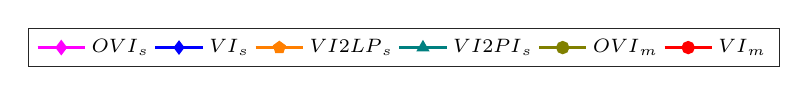
\begin{tikzpicture}
\begin{axis}[width=0.8\textwidth, height=0.2\textwidth, hide axis, xmin=0, xmax=10, ymin=0, ymax=0.2,legend columns=6, 
            legend style={draw=white!15!black,legend cell align=left, at={(0.5,0.5), font=\scriptsize}},]
    \addlegendimage{colstormovi, mark=diamond*, thick, mark options={solid,scale=1.1}}
    \addlegendentry{$\text{OVI}_\tool{s}$}
    \addlegendimage{colstormvi, mark=diamond*, thick}
    \addlegendentry{$\text{VI}_\tool{s}$}
    \addlegendimage{colstormlp, mark=pentagon*, thick}
    \addlegendentry{$\text{VI2LP}_\tool{s}$}
    \addlegendimage{colstormpi, mark=triangle*, thick}
    \addlegendentry{$\text{VI2PI}_\tool{s}$}
    \addlegendimage{colmcstaovi, mark=*, thick}
    \addlegendentry{$\text{OVI}_\tool{m}$}
    \addlegendimage{colmcstavi, mark=*, thick}
    \addlegendentry{$\text{VI}_\tool{m}$}
    
\end{axis}
\end{tikzpicture}
}


